%!TeX program=pdflatex
%!TeX encoding=utf8
%!TeX spellcheck = en_GB
%!TeX root = ../../messageVortex.tex

\part{Results}
To verify the hypothesis made in this paper, and to analyse properties of the protocol in a real world scenario a library was implemented in Java which was capable of handling all message packets and the routing stack as a whole. The following paragraphs describe the protocol developed in general as a generic approach. Appendix \ref{app:asnone} gives the full ASN.1 representation of the protocol. 

It is important to notice that ASN.1 has no mean to express encrypted structures. Due to this fact we defined all encrypted fields as \verb|OCTET STRING|. 

The protocol is defined int the ASN.1 to support onionized information in an unencrypted form. This is meant for debugging purposes only. At no point should this possibility be used in a production environment.

The protocol described in the next chapter is independent from routing. We built a blending layer for SMTP. Layers for other protocols such as XMMP may be built similarly. The protocol may be extended by adding blending layers and their addressing schemes.

The Protocol outlined here is the final product and has undergone many development cycles. A lot of really useful features and capabilities such as a mechanism analoguous to the SMTP received headers were dropped as they were very useful but threatened security or anonymity.

\chapter{Protocol Overview}
The MessageVortex protocol described here is an onionizing protocol for asynchronus data transfer. The protocol itself is embbeded into a carrier protocol as binary information to avoid easy detection and make it hard to block traffic without blocking other legitimate traffic.

The data transferred is passed thru a number of mixes. The builder of a routing block (normally the sender) decides upon the following attributes:
\begin{itemize}
	\item Hops for the message and all decoy traffic.
	\item Timing behaviour respectively speed of the message.
	\item Decoy traffic generation.
	\item Set of possible recipients.
\end{itemize}

These decisions are compiled into a routing block structure which is onionized. This routing block may then be used to transfer a message of almost any size. This message is then sent to the involved mixes.

A mix may be just an intermediate station or the final target of a message. Only the recipient of a message is able to tell whether a message was intended for him or not. Any mix does a certain number of operations on a message. Considering the message, the timing and the operations applied a mix may extract the following informations:

\begin{itemize}
	\item IP of the sending mix.
	\item Size of the message received.
	\item Size of all processed sub blocks.
	\item Arrival time of a message.
	\item Ephemeral identity a message belongs to (ephemeral pseudonym to the routing block builder).
	\item Validity time of the message on the node.
	\item Operations applied to the message.
	\item Size of all blocks sent.
	\item IPs of the receiving mixes.
\end{itemize}

A mix always applies the operations requested in the building instructions to the received data. If this is not done properly the message may fail to transfer to its final destination. 

The operations to be applied on a message are chosen in such a way that they may or may not generate decoy traffic. This guarantees that a valid message may not be identified on the operations applied to the message.

Redundancy may be built in a routing block as well as progress indication.

\section{Vortex Message}
The following outline is a simplified view onto the message block of MessageVortex.

\begin{figure}[hbt]
	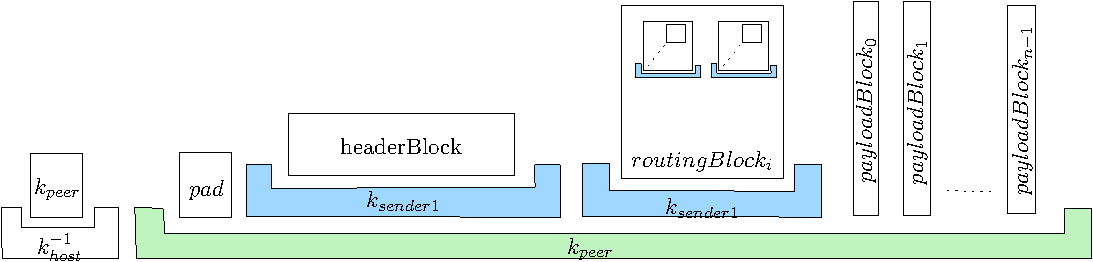
\includegraphics[width=\textwidth]{inc/blockLayoutSimplified}
\end{figure}

A vortex message is a message passed from one mix to another this message may or may not contain any valuable information. The message itself is embedded as binary data into a transfer protocol. Every Mix may decide for himself what kind of protocols and embedding mechanisms are supported.

A vortex message is always built out of these blocks:
\begin{itemize}
	\item header
	\begin{itemize}
		\item Encrypted message key.\\
			  Contains symmetrical key for decryption of follow up header information and payload blocks. Encrypted with host identity public key.
		\item Identity and ``proof of work'' information\\
		      Contains Requests, Proof of work sections, and header key
	\end{itemize}
	\item Encrypted payload blocks (encrypted with header key)
	\begin{itemize}
		\item Routing blocks (encrypted with message key)
		\begin{itemize}
			\item Next hop timing instructions
			\item Next hop routing blocks (encrypted)
			\item Next hop header
			\item Message build instructions.
			\item Next hop header key and spec.
			\item Next hop blending instructions.
		\end{itemize}
		\item Payload chunk blocks
	\end{itemize}
\end{itemize}

It is important to note that there are two symmetrical keys involved in encrypting and decrypting message headers. This is not a flaw in the protocol but necessary. 

The first key which is in a Vortex message is the message key. This key is only accessible with the private key of the node receiving the message. It allows decryption of the routing blocks and the header information. The sender of a message block is therefore not able to tell if a message contains one or more routing blocks. It is important to note that no other node should have access to this information. 

The second key is the header key located in the encrypted header. This key was chosen by the creator of the routing block containing the information. This key protects the inner structure of the Message. it makes it impossible for any node except the sending or the receiving node to detect the inner structure of the message. Without this key any independent observer with knowledge about the blending capabilities of a receiving node may;
\begin{itemize}
	\item easier identify the block structure.\\ 
	This remains the case regardless whether ASN.1 or length prefixed structures are used. If the structure of a vortex Message can be easily identified the messages may be logged or dropped.
	\item Identify the routing block size.\\
	The value of this information is only very limited as it only reflects indierctly the complexity of thr remaining routing information.
	\item Identify the number of payload blocks and their respective sizes. \\
	This is valuable information when following a traffic.
\end{itemize}

\subsection{Key Usage}
\fxfatal{add content here}

\subsubsection{Message Key}
\fxfatal{add content here}

\subsubsection{Header Key}
\fxfatal{add content here}

\subsubsection{Identity Key}
\fxfatal{add content here}

\subsubsection{Ephemeral Identity Key}
\fxfatal{add content here}

\subsection{VortexMessage Processing}
\subsubsection{Receiving Messages}
All messages are processed as follows:
\begin{enumerate}
	\item Extract length prefixed message key from block. Abort if not decryptable or invalid block.
	\item Decrypt message key with hosts private key $\rightarrow$ message key
	\item Extract length prefixed header message. Abort if too big.
	\item Decrypt header block with decrypted message key. Abort if not decryptable or invalid block.
	\begin{itemize}
		\item Verify identity
		\item Check quotas (if any)
		\item Extract header key
		\item Extract requests (if any)
		\item Check replays (if any)
	\end{itemize}
	\item Decide if message should be processed. If not abort here.
	\item Decrypt main block with message key
	\item Extract payload chunks.
	\item decrypt routing blocks with header key.
	\item Check backref secrets.
\end{enumerate}

Every routing block creates a new message.

The payload of a message is generated according instructions in the routing block. Timing instructions are relative to the arrival time of the message containing the routing block. This is necessary as a routing block may be used multiple times (see section \ref{sec:murb}).

A vortex message may be composed not earlier than a ``validFrom'' expressed in the respective routing block.

\subsubsection{Building and Sending Messages}
Any time after a routing block reaches ``vakidFrom'' and before the ``validTo'' is reached processing of a routing block is triggered. An implementation should when triggering a routing block for processing trigger as many routing blocks as possible to make traffic analysis harder.

The message is then built as follows:
\begin{enumerate}
	\item Check if all building instructions can be fulfilled due to their prerequisites.
	\item Build requested payload blocks.
	\item Extract message key from routing block.
	\item Extract headerBlock from routing block.
	\item Extract (message key encrypted) nextHop routing blocks from routing block.
	\item Encrypt main block (routing blocks and payload blocks).
	\item Update accounting figures.
	\item Blend into transport layer and send message.
\end{enumerate}

\fxfatal{add more details about sending and blending}

\subsection{VortexMessage Operations}
All operations are expressed as described in section \ref{sec:buildInstr}. The following sections give important details about the implementation of the operations.

\subsubsection{VortexMessage SplitPayload Operation}
The splitPayload operation splits a payload block into two chunks of different or equal sizes. The parameters for this operation are:

\begin{itemize}
	\item source payload block $pb_1$
	\item fraction $f$\\
	      Floatingpoint number describing the size of the first chunk. If fraction is 1 then the whole payload is transferred to the second target chunk
\end{itemize}

If $len(pb_1)$ expresses the size of a payloadblock called $pb_1$ in bytes then the two resulting blocks of the SpitPayload Operation $pb_2$ and $pb_3$ have to follow the following rules:

\begin{eqnarray}
split(f, pb_1) & = &\langle pb_1, pb_2 \rangle\\
pb_1.startsWith(pb_2)\\
pb_1.endsWith(pb_3)\\
len(pb_2) & = & floor(len(pb_1)\cdot f)\\
len(pb_1) & = & len(pb_2) + len(pb_3)
\end{eqnarray}

\fxfatal{add section about fp implementations and constraints for implementations}

\subsubsection{VortexMessage MergePayload Operation}
The mergePayload operation combines two payload blocks into one. The parameters for this operation are:

\begin{itemize}
	\item first source payload block $pb_1$
	\item second source payload block $pb_2$
\end{itemize}

If $len(pb)$ expresses the size of a payloadblock called $pb$ in bytes then resulting block of the MergePayload Operation $pb_3$ have to follow the following rules:

\begin{eqnarray}
merge(pb_1, pb_2) & = & pb_3 \\
pb_3.startsWith(pb_1)\\
pb_3.endsWith(pb_2)\\
len(pb_3) & = & len(pb_1) + len(pb_2)
\end{eqnarray}

\subsubsection{VortexMessage XorSplitPayload Operation}
The xorSplitPayload operation forks payload block into two payload blocks. The parameters for this operation are:

\begin{itemize}
	\item Source payload block $pb_1$
	\item fraction $f$
	\item PRNG Initializer $pi$
\end{itemize}

If $len(pb)$ expresses the size of a payloadblock called $pb$ in bytes then resulting block of the MergePayload Operation $pb_3$ have to follow the following rules:

\begin{eqnarray}
xorSplit(pb_1, f, pi) & = & \langle pb_2,pb_3 \rangle \\
pb_2 & = & prng( i, floor(len(pb_1)\cdot f) )\\
pb_3 & = & pb_1 \oplus pb_2\\\
len(pb_2) & = & floor(len(pb_1)\cdot f)\\
len(pb_3) & = & max( len(pb_1), len(pb_2) )
\end{eqnarray}

\fxfatal{add reference fp implementations and constraints}

\fxfatal{add reference to the PRNG section}

\subsubsection{VortexMessage XorMergePayload Operation}
The xorSplitPayload operation forks payload block into two payload blocks. The parameters for this operation are:

\begin{itemize}
	\item First source payload block $pb_1$
	\item Second source payload block $pb_2$
\end{itemize}

If $len(pb)$ expresses the size of a payloadblock called $pb$ in bytes then resulting block of the xorMergePayload Operation $pb_3$ have to follow the following rules:

\begin{eqnarray}
xorMerge(pb_1, pb_2) & = & pb_3 \\
pb_3 & = & pb_1 \oplus pb_2\\\
len(pb_3) & = & max( len(pb_1), len(pb_2) )
\end{eqnarray}


\subsubsection{VortexMessage EncryptPayload Operation}
The encryptPayload operation encrypts a payload block $pb_1$ symmetrically resulting in a block $pb_2$. The length of block $pb_2$ may vary according to mode and padding chosen. The parameters for this operation are:

\begin{itemize}
	\item Source payload block $pb_1$
	\item Encryption specification $spec$
	\item Symmetric key $k$
\end{itemize}

The operation follows the following rules (please note section \ref{sec:encNot} for notation):
\begin{eqnarray}
encrypt(pb_1, spec, k) & = & pb_2 \\
pb_2 & = & E_{spec}^{K_a}\left( pb_1 \right)\\\
len(pb_2) & \geq & len(pb_1)
\end{eqnarray}


\subsubsection{VortexMessage DecryptPayload Operation}
The decryptPayload operation decrypts a payload block $pb_1$ symmetrically resulting in a block $pb_2$. The length of block $pb_2$ may vary according to mode and padding chosen. The parameters for this operation are:

\begin{itemize}
	\item Source payload block $pb_1$
	\item Decryption specification $spec$
	\item Symmetric key $k$
\end{itemize}

The operation follows the following rules (please note section \ref{sec:encNot} for notation):
\begin{eqnarray}
decrypt(pb_1, spec, k) & = & pb_2 \\
pb_2 & = & D_{spec}^{K_a}\left( pb_1 \right)\\\
len(pb_2) & \leq & len(pb_1)
\end{eqnarray}

\subsubsection{VortexMessage addRedundancy Operation}
\fxfatal{add content here}

\subsubsection{VortexMessage removeRedundancy Operation}
\fxfatal{add content here}



\section{VortexMessage Request Processing}
Vortex message requests allow a Vortex node to gain knowledge about the Vortex network and create new identities.

\fxfatal{add content here}

\subsection{VortexMessage Requests}
These requests are contained in the header portion of a Vortex message. These requests are purely for bootstrapping and maintaining the quota system and for requesting network capability.

The request information is defined in section \ref{sec:request}. For more information about the exact binary representation of all blocks and data see chapter \ref{sec:spec}.

Any node decides on its own what type of requests are being answered. 

A node not replying to clear text request is called a ``stealth node'' (see \ref{sec:stealthNode}). Such a stealth node discloses itself only to participants which do allready know at least the public key of the node. This usually means that they have ``earned'' this information by issuing a queryPeer request to another node and obtaining the information did already generate costs to the sender.

A node only replying to a fixed set of identities (in that specific case they are not ephemeral) is called a ``hidden node'' (see section \ref{sec:hiddenNode}).

It is recommended that unencrypted requests are not answered. A node may decide to answer unencrypted queryCapability requests in order to enable clients to bootstrap without (or with a minimal) network knowledge.

If a message contains $n$ requests in a header block it must supply at one reply blocks at the beginning of the routing block list. All reply blocks are concatenated and sent using the reply block. If the first block in the routing block list is not a reply block the request will fail.

\subsubsection{QueryCapability Request}
This request is primarily used to initialize a conversation with a node. It contains valuable information about the capability of the node as well as information about the embedding supported or the encryption. A node may or may not reply to a queryCapability requests. Doing so confirms the node to be participating in the vortex network.

The only valid reply is a replyCapability message in encrypted form.

\subsubsection{NewIdentity Request}
If this request is accepted it generates a new ephemeral identity. The identity itself is stored in the header fields. The standard behaviour is to reply with a replyPuzzleRequired block. 

This request generates a temporary ephemeral identity for the limited time denoted in the validity field of the reply block. No quota is assigned during that phase. As soon as the identity offers a valid puzzle solution the requested quota is assigned and the identity may be used for subsequent requests.

If a puzzle is not solved within the given time the temporary identity may be deleted. A node should not accept a solved puzzle after the given duration. 

Request with too high message or transfer quota requests should be answered with an replyPuzzleRequired block containing a zero length puzzle.

\subsubsection{QueryPeer Request}
As outlined in section \ref{sec:request} this request should be very costly and harvesting of known addresses should be hard. Furthermore this request should always  disclose the nodes from a fixed subset of the nodes known to the queried mix. This maximizes the effort to harvest participating nodes.

It is at the same time worth mentioning that this limit may opose a thread that traffic is concentrated on similar nodes within participating nodes using the same initial set of known addresses to bootstrap. This due to the fact that if using the same node to bootstrap for multiple participants within a group results in peer knowledge which is similar. thus resulting in a similar network. It is however also worth mentioning that participants belonging to more than one group will evolve over time as their different peer partners will result in different anonymity sets over time even when aplying exact the same anr reproducable rules.

\fxfatal{integrate sec query section from GIT here}

\subsubsection{TransferQuota, MessageQuota,  and QueryQuota Request}
This request may be accepted by a node if and only if the sender is a valid identity. It may be accepted even for a temporary identity.

The transfer quota offers the capability to raise the number of bytes an identity may transfer. This quota may be risen at any time. It is up to the owner of an ephemeral identity and the node using the identity to decide whether an identity may be kept or not respectively its quotas raised.

The Message Quota is a quota not limiting the number of bytes but the number of messages. As every message generates accounting overhead this number has to be limited as well. There are constraints similar to transferQuota when raising this value.

The queryQuota request enables the owner of an identity to query the current amount of remaining messages respectively bytes.

\subsection{VortexMessage Reply Blocks}
Reply blocks are as outlined in section \ref{sec:replyBlock} prefixed payload blocks. All reply blocks except the ctxless\ldots reply blocks are a result of a header request.

\subsubsection{ReplyCapability block}
The replyCapabilityBlock is the reply block to a queryCapability Request. The information provided here is outlined in section \ref{sec:replyBlock}. It is important to note that this block is even when requested in plain is always onionized and thus unreadable for third parties. 

A node may offer different capabilities to known identities than to anonymous clear text requests.

\subsubsection{replyPuzzleRequired block}
The replyPuzzleRequired block is the block reflecting the payment for a requested operation such as newIdentity, queryPeer, transferQuota, or messageQuota request.

Every puzzle block will create an accounting entry as outlined in section \ref{sec:accounting}. 

A node may reject an operation for any reason including exceeding an unnatural ammount of outstanding puzzles.

A reply containing a null length puzzle means that the requested operation is rejected.

\fxfatal{This block will change as new proof of work are introduced. The same applies to the respective header section}

\subsubsection{replyStatus block}
\fxfatal{This block will possibly disapear}

\subsubsection{CtxlessNewidentity block}
Th new identity block is to propagate a newly generated, non-ephemeral identity of a user. This block should not be ignored by any node. It enables a user to strengthen its identity. 

It is however should ignore the request if its acceptance results in a reduced security lavel of the current identity.


\chapter{Vortex Prerequisites}
\section{Hardware}
No special Hardware is required for running Vortex nodes. The capabilities of Vortex are designed in such a way that ordinary mobile phones may act as vortex nodes. It is however recommended to have a node always connected to the internet. A mobile phone may disconnect from time to time based on the availability of the network. For our experiments we use a RaspberryPi Version 1. It is however recommended to use a faster, newer model due to the memory requirements of the proof of work.

\fxfatal{add more content here}

\subsection{Considerations Regarding Weak or Unsuitable Hardware}
\fxfatal{add more content here}

\section{Addresses}
A Vortex address is built as follows: $vortexAddress=<transport>:<address>!<publicKey>$

To allow storage of Vortex addresses sin standard messaging programs such as Outlook or Thunderbird. We define an alternate representation $encodedVortexAddress=base64(<transport>:<address>).<publicKey>@localhost$. 

The suffix ``@localhost'' makes sure that a message intended for Vortex is not routed by any non-participating server.

The main downside of vortex addresses are that they are no longer readable by a human. The main reason for this is the public key which is required. We may abstract this further by allowing clear text requests on the main email address for the public key. Such requests must then be answered by the vortex account with the valid Vortex address.

\subsection{Public Key Encoding in Address Representation}
The public key of an address is encoded as follows:
\begin{enumerate}
	\item The asymmetric key is encoded as specified in the AsymmetricKey in ASN.1
	\item The ASN.1 representation is then encoded using BASE64
\end{enumerate}	

\section{Transport Layers}
As transport layer protocols we specified the protocols SMTP and XMMP as valid transport layers. In the following sections we specify the transport properties for these protocols.

\subsection{SMTP}
In SMTP we defined ``smtp'' (lower case) to be the transport specifier. When using SMTP messages are always encoded as attachments. 

If not further specified by the receiving node an attachment should be the encoded message. 

Valid properties may be:
\begin{itemize}
	\item Encoding $"encoding="("plain:"<numberOfBytesOfOffset>[,<numberOfBytesOfOffset>]*|"f5")$
\end{itemize}

All SMTP nodes responding to clear text should at least support $encoding=plain:0,1024$.

\fxwarning{do layout here}

\subsection{XMMP}
\fxfatal{add more content here}

\section{Client}
We did not create a Vortex client for sending messages. Instead we used a standard Thunderbird email client pointing to a local SMTP and IMAP Server provided by Vortex. On the SMTP side Vortex does encapsulate where possible mails into a Vortex message and builds automated route to the recipient. The SMTP part of vortex may be used to encapsulate automatically all messages with a known Vortex identity into a vortex message. On the IMAP side it merges a local Vortex message store with the standard Email repository building a combined view.

Using Vortex like this offers us the advantages of a known client with the anonymity Vortex offers.

This has certain downsides. At the moment the vortex client has only a local store this makes it impossible to handle multiple simulatneously connected clients to use Vortex. This is however just a lack of the current implementation and not of the protocol itself as we may safely use an IMAP storage for storing vortex mails centrally.

\subsection{Vortex Accounts}
By definition any transport layer address may represent a Vortex identity. This fact may make people believe that their current email or jabber address is suitable as Vortex address. This is technically perfectly true, but should not be done for the following reasons:

\begin{itemize}
	\item If an address is identified as a vortex address it may be blocked (directly or indirectly) by an adverser.
	\item If a vortex node is malfunctioning non-vortex messages should remain unaffected. This is more likely to happen if non-Vortex messages are kept in a separate account.
	\item If a user wants no longer to maintain its Vortex address (hopefully there will be a better technology in future) he just may give up his Vortex accounts. If he would have been using his normal messaging account for Vortex he would receive mixing messages which he has to filter in future.
\end{itemize}

\subsection{Vortex Node Types}

\subsubsection{Public Vortex Node}
Public nodes are nodeswhich advertise themself as mixes. Just as all nodes they may be an endpoint or a mix. Typically they accept all requests exactly as outlined in \ref{tab:protoReplyCrit}. As an immediate result of the publicly available information about such a node the owner may be target of our adverser. Pressure may be oposed to close down such a node. However since we do not need a specific account we may safely close down one transport account and open up a different one (on the same or a different infrastructure).

\subsubsection{Stealth Vortex Node\label{sec:stealthNode}}
This node does not answer any clear text requests. As an immediate result the node is only usable by other nodes knowing the public key of this node. The node is therefore on a known secret base only reachable.

\subsubsection{Hidden Vortex Node\label{sec:hiddenNode}}
A hidden node is a special form to a stealth node it has a set of preset identities. Only these entities are processed. This behaveour has certain drawbacks. An identity may not be changed. As an immediate result traffic may become a pseudonymity. To counter this effect at least partially we may use the same local identity for multiple senders. As an immediate result the sender is only one of all senders knowing the private key of an identity.

\chapter{MessageVortex - Transport Independent Messaging anonymous to \nth{3} Parties\label{sec:spec}}
This approach is different from all approaches discussed previously. Unlike them we put complete distrust into the infrastructure being used. Furthermore we do not rely on a custom server infrastructure in the internet. Instead we take advantage of the availability of internet connected devices such as internet connected mobile phones, tablets, or even commonly available SoC such as RaspberryPi or similar. It is still very hard to maintain a server in the internet and considering the vastly growing amount of automated attack carried out against internet connected servers it is not advisable or realistic to assume that a future user of this system owns either a server or connects to a service which is offering explicitly anonymizing services. These infrastructures would be suspectible to monitoring or even banning. Instead we take a different approach.

We use common messaging protocols as transport layers and connect to them using the respective client protocols. The actual mixes are operated by the users on their ``always connected'' devices. It goes without saying that such a system is far less reliable than a traditionally run server as this hardware is typically cheap and normally connected to the internet using a bandwidth shared media.

The basic idea is that a client generates all traffic (including decoy or dummy traffic) by itself. It defines the routes a message takes through the mixes and decides which targets are receiving dummy traffic at the same time. In such a system even when possessing all the nodes routing the traffic (without the endpoints) an anonymity set of $k$ (whereas the size of $k$ is defined by the sender) is guaranteed.

As decoy traffic is generated with the same operations as the true content is split it is impossible for an adverser running a node to determine whether he is generating noise or actually processing the true message.

\fxfatal{add a lot more text here}
\begin{figure*}[h]
	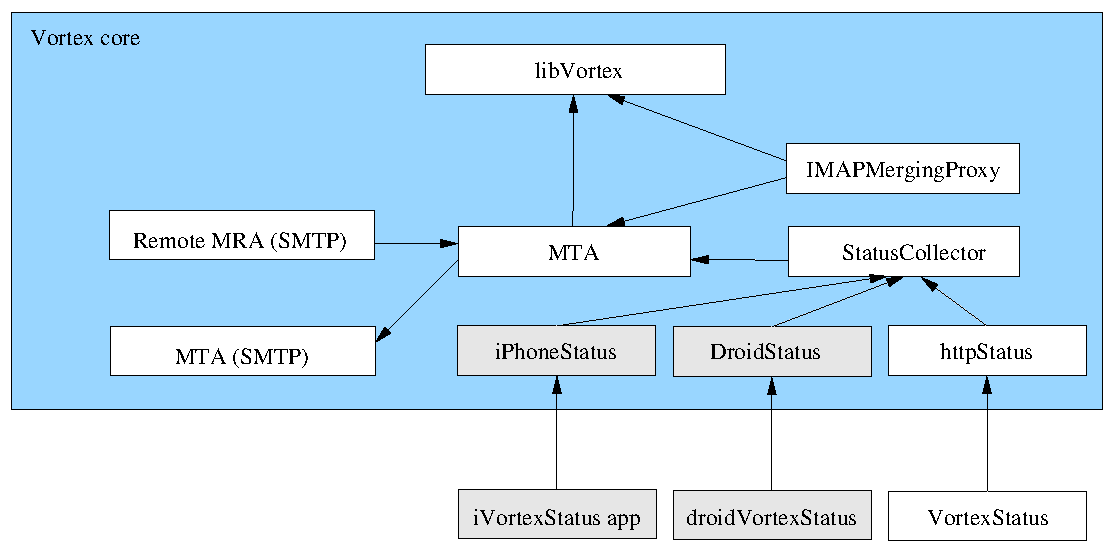
\includegraphics[width=\textwidth]{inc/VortexModules.pdf}
	\caption{Overview of the Vortex modules}
	\label{fig:vortexModules}
\end{figure*}
\fxfatal{replace image with up to date representation; show implemented and not implemented parts; Maybe make it two column wide}

\section{Protocol Implementation\label{protoImpl}}
\fxfatal{add content here}

\section{Block Structure}
\lstinputlisting[language=ASN1, caption={Header Block}, backgroundcolor=\color{gray!10},linerange={29-71},firstnumber=29]{../app/asn.1/messageBlocks.asn} 

\subsection{Header Block}
\fxfatal{add content here}

\subsection{Routing Blocks}
\fxfatal{add content here}

\subsection{Payload Blocks}
\fxfatal{add content here}

\section{Message Building}
\fxfatal{take care of percentage and floating point precision}


\section{Accounting}
In table \ref{tab:protoReplyCrit} we show under what circumstances a reply to a header request should be sent. The capitalised words MAY, MUST, SHOULD and SHOULD NOT are used as defined in RFC2119\cite{RFC2119}.
\begin{table*}[h]
	\centering\scriptsize
	\begin{tabular}{|l|l|l|l|l|}\hline
		\diaghead{\theadfont Request Criteria}{Request}{Criteria} & \thead{unknown identity; cleartext} & \thead{unknown identity; encrypted} & \thead{expired identity; encrypted} & \thead{known identity; encrypted}\\\hline
		newIdentity	 	& SHOULD NOT 	& SHOULD NOT& Invalid (Error) 	& Invalid (Error)\\              
		queryPeer       & MUST NOT      & MUST NOT  & MAY               & MAY\\        
		queryCapability	& SHOULD 		& MUST 		& MUST				& MUST \\
		messageQuota	& MUST NOT 		& MUST NOT	& MAY				& MUST \\              
		transferQuota	& MUST NOT		& MUST NOT	& MAY				& MUST \\\hline             
	\end{tabular}	
	\caption{Requests and the applicable criteria for replies}
	\label{tab:protoReplyCrit}
\end{table*}

\fxfatal{add content here}

\section{Blending layer}
In our implementation the blending layer is a weak implementation. It attaches a message in non-obfuscated form with a mime type application/octet stream the application name is randomly chosen. Start offset is fixed to 200 and a valid header part is prepended. Text is not generated.

\fxfatal{add text about why the sender may not control this layer completely}

\fxfatal{add misuse to create virus attachment if headerless plain}

\fxfatal{add parrot circumvention}

\fxfatal{add content here}

\subsection{Plain Inclusion}
\fxfatal{add about }

\subsubsection{File Type Candidates}

\fxfatal{add content here}

\subsection{F5 Steganography}

\fxfatal{add content here}

\section{Message Flows}

\fxfatal{add content here}

\section{Considerations for Building Messages}
In a worst case scenario we assume that an adverser is controlling most of the network utilized for anonymisation. While this is not necessarily a problem (as pointed out earlier) it allows an adverser to track a message while agents are being used under his control. So for simplicity and as a worst case assumption we always assume that an adverser has perfect knowledge of an associated message flow. This is however a worst case scenario. One missing agent disconnects the whole chain and as messages are not traceable in size.

\fxfatal{add selffailing operations as checkpoint}

\subsection{Ephemeral identities}
\fxfatal{expiring ephemeral identities should not only be replaced after their expiration but anytime during the livetime}

\subsection{Timing of messages}
\fxfatal{add content here}

\subsection{Diagnostics}
\fxfatal{add content here}

\fxfatal{add here why is there no hashing operation (makes traffic distinguishable)}


\subsubsection{Implicit Diagnostic}
\fxfatal{Add comments about messages splitting and returning to sender}

\subsubsection{Automatic Explicit Diagnostic}
\fxfatal{Add comments about error and diagnosis messages officially spliting of messages}

\subsubsection{On-Demand Explicit Diagnostic}
\fxfatal{Add comments about normal, error, and diagnosis messages being picked up by a routing block}

\section{Verification of requirements}
In the previous sections we identified the following list of requirements:

\slistofrequirements

In the following subsections we will iterate through all requirements and verify to what degree we achieved the goal.

\fxfatal{list all requirements}

\paragraph*{\ref{req:zeroTrust}:} 
We have not put any trust into an external infrastructure. While we do assume that all routing nodes act as defined. A misbehaving node may be identified and eliminated without putting any trust on other nodes. Analysis have shown no means for a misbehaving node which might be intentional or unintentional endangering anonymity at any time. We do not rely on any third party technology or infrastructure for our anonymity. 

This requirement is therefore fulfilled.

\paragraph*{\ref{req:P2P}:} 
No node has additional privileges or offers additional services. All are equal and share the same privileges.

This requirement is therefore fulfilled.

\paragraph*{\ref{req:untagable}:} 
Messages may not be tagged. All content is either strictly onionised or defined and linked with unknown hooks. Tampering with a message will cause the message delivery to fail at the next node.

This requirement is therefore fulfilled.
 
\paragraph*{\ref{req:unbugable}:} 
There are always means to bug a message. As we put trust in sender and recipient and we know already that a intermediate mixing node is not able to modify the message the protocol is hard to bug. There may be a possibility to bug a message with a routing log entry over DNS. If a recipient is not resolving names or trusts in the content of such a message he is safe.

This requirement is therefore fulfilled. May be only partially fulfilled if log entries are not handled with care.

\paragraph*{\ref{req:replay}:} Messages may only be replayed a limited amount of times. The number of replays is controlled by the sender and may not be altered by any mix. A malfunctioning mix replaying more often than allowed will not be able to extract any information than the information it obtained when sending the first time. 

This requirement is therefore fulfilled.

\paragraph*{\ref{req:accounting}:} 
All identities generated are not traceable as any identity is generated without any context and may not be mapped to an older or newer identity (perfect anonymous forward identity). Neither the source nor the replies may be used to be traced as all messages 

This requirement is therefore fulfilled.

\paragraph*{\ref{req:anon}:} This point is the hardest to proof. We certainly achieved a high degree of anonymity. No node can tell by observing traffic if a node is a final recipient or just a mix. There are however some weaknesses in the protocol. As the implementation is currently connecting simultaneously to the true name (email or jabber account in the current implementation) and the Vortex account the user might be identified by that fact. Using a anonymisation proxy could solve the problem but it would violate the Zero trust principle.

This requirement is therefore only partially fulfilled. However, the weakness is very faint.

\paragraph*{\ref{req:boot}:} 

\fxfatal{add content}
\paragraph*{\ref{req:cryptVar}:} 

\fxfatal{add content}

\paragraph*{\ref{req:easy}:}

\fxfatal{add content}

\section{Considerations for Routing Messages}
\subsection{Time of sending}
Messages should always be sent timewise nearby other messages. This means that the best moment for sending a message in a ready queue is at a time when sending of other messages is due. However no optimisation should be done to send as many messages as possible at the same time. this would lead to a forseeable behaviour of the routing layer and thus to misusable behaviour.

\section{Real World Considerations}
This approach is heavily dependent of the transport protocol and builds on top a new obfuscating/routing layer. For this system to become a real peer-to-peer approach some additional quirks are required. A message-Vortex-Account needs always an active routing handler. This routing handler may be introduced by new server capabilities or by having a device handling the routing from the client side. For this reason we built a RaspberryPi appliance capable of connecting to one (or more) accounts fetching incomming mails, analysing them and reroute them if necessary. Although the system is designed to be run on a RaspberryPi the software might be installed to any Java capable client. The RaspberryPi is just one affordable lightweight device which offers all required capabilities.

\subsection{No Routing Log}
There was up until very late a routing log functionality in the protocol. This functionality did however have the disadvantage that it allowed bugging and could possibly  disclose intermediate mixes to a recipient which did not comply with the policy the mixes might have chosen. Therefore this feature was dropped and replaced with the fetch block behaviour.

\subsection{No Verification Possibilities}

\subsection{Very Limited Control Blending Layer for the sending node}

\subsection{Message Content}
\fxfatal{add content here}

\chapter{Security Analysis}
In the following sections we emphasize on attacks targeting either sender recipient tuples or on identification of participants. 

Based on the protocol we may safely assume the following key ponts:
\begin{itemize}
	\item An adverser knows and controls a significant number of nodes (for our analysis we assume less than 80\%).
	\item An adverser may observe the traffic at any point without getting any information about the message content
	\item An adverser is not capable of matching multiple messages on different nodes to one message.
\end{itemize}

We always assume an adverser to have more knowledge than we think he may extract from the messages.
\begin{itemize}
	\item We assume that an adverser knows all messages of a transaction running over his nodes and matches them correctly to the same message.
	\item 
\end{itemize}

We assume that the adverser is targeting the following informations:
\begin{itemize}
	\item Sender identity
	\item Recipient identity
	\item Message content
	\item Message size
\end{itemize}

\section{Attack on Users Identity}
\fxfatal{add content here}

\subsection{Frequency and Bandwidth Analysis}
\fxfatal{add content here}

\section{Attack on Message content}
\fxfatal{add content here}

\subsection{Attacking Routing Blocks}
\fxfatal{add content here; Routing block length analysis}

\section{Attack on Message size}

\fxfatal{add content here}

\chapter{Additional Considerations}
\section{Man in the Middle Attacks to Conversations}

\fxfatal{add content here}

\section{Identification of Participating Accounts}

\fxfatal{add content here}

\subsection{Identification by Content}
It is possible to identify a message by content. Assuming that an adverser knows the applied blending methode he may identify an ASN.1 structure of 

\fxfatal{add content here}

\subsection{Identification by Query}

\fxfatal{add content here}

\subsection{Identification by Traffic Type}

\fxfatal{add content here}

\subsection{Identification by Bandwidth}

\fxfatal{add content here}

\subsection{Identification by Behavioural Analysis}

\fxfatal{add content here}

\section{Storage of Messages and queues}
The storage of messages sent though MessageVortex should be handled with great care. It seems on the first sight a good idea to merge all messages in a globally available storage such as the IMAP account of the receiving entity. However -- In doing so we would discover the message content to the providing party of a mail account. Since we handled the message with great care and tremendous costs up until this point it would be careless doing so. 

Storing them in a localized and receiving entity controlled storage is definitely a good idea but leaves security considerations like a backup possibly to an end user. This might be better, but in effect a questionable decision. There is however a third option. By leaving the message unhandled on the last entity of the MessageVortex chain we may safely backup the data without disclosing the message content. Merging the content then dynamically through a specialized proxy would allow the user to have a unified view on his without compromising the security.

\fxfatal{implemented in prototype?}

\section{Economy of transfer}

\fxfatal{Write something about wasting bandwidth}